\section{Exploratory Data Analysis}
\label{sec:eda}

All figures are produced by \texttt{report/scripts/make\_figures.py} from
the cached 2018-02-20 batch (\texttt{u1}), using its 39 cells with a valid
cycle life.

\subsection{Capacity fade}
Fig.~\ref{fig:fade} plots discharge capacity against cycle number for all
39 cells, coloured by cycle life. Three features stand out:
\begin{itemize}
  \item \textbf{The knee.} Capacity stays nearly flat (about 1.07--1.11\,Ah)
  for most of the cell's life, then drops sharply. Before the knee, a
  long-lived cell and a short-lived cell look almost the same. This is why
  capacity alone is a poor early predictor.
  \item \textbf{Two clusters.} The standard cells fail between cycles 392
  and 514. The \texttt{-newstructure} cells fail between cycles 777 and
  1186.
  \item \textbf{Early rise.} Many standard cells gain a little capacity over
  roughly the first 100--200 cycles before fading. This is commonly
  reported for LFP/graphite cells.
\end{itemize}

\begin{figure}[t]
  \centering
  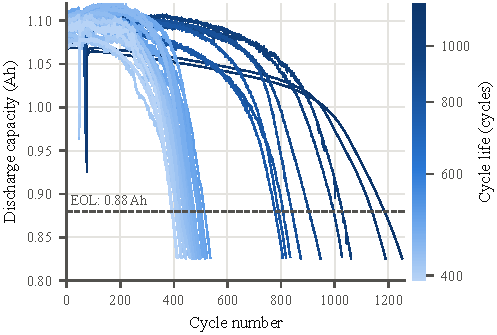
\includegraphics[width=\columnwidth]{fig_capacity_fade}
  \caption{Discharge capacity against cycle number for the 39 cells, coloured
  by cycle life (log scale). The dashed line is EOL (0.88\,Ah, 80\% of
  nominal). The sharp single-cycle dips are measurement artefacts.}
  \label{fig:fade}
\end{figure}

\subsection{Cycle-life distribution}
Fig.~\ref{fig:hist} shows that the cycle-life distribution has two separate
peaks. The 30 standard cells average 453 cycles and the 9
\texttt{-newstructure} cells average 942 cycles; no cell lies between 514
and 777 cycles. Fig.~\ref{fig:policy} breaks cycle life down by policy.
Among standard cells, two patterns appear:
\begin{itemize}
  \item The shortest lives (about 390--420 cycles) come from policies that
  either start slowly and finish at high current (\texttt{3.6C(9\%)-5C},
  \texttt{3.6C(30\%)-6C}) or use the most extreme first step
  (\texttt{6C(60\%)-3C}).
  \item Moderate policies, such as \texttt{4.8C(80\%)-4.8C} and
  \texttt{5.2C(58\%)-4C}, reach about 480 cycles.
\end{itemize}
Cells charged with the same policy still differ by up to about 80 cycles,
which is the cell-to-cell variation that makes prediction difficult.

\begin{figure}[t]
  \centering
  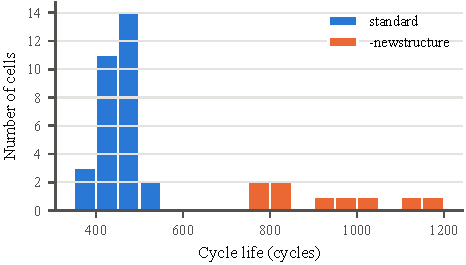
\includegraphics[width=\columnwidth]{fig_life_hist}
  \caption{Histogram of cycle life, stacked by group.}
  \label{fig:hist}
\end{figure}

\begin{figure}[t]
  \centering
  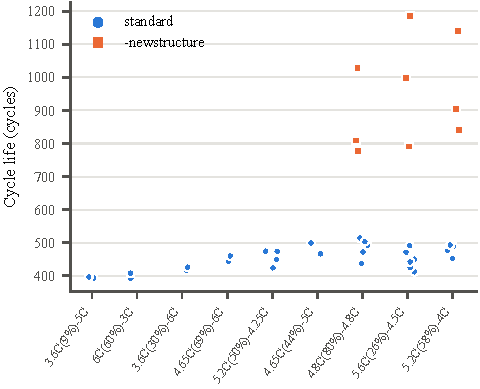
\includegraphics[width=\columnwidth]{fig_life_by_policy}
  \caption{Cycle life of each cell grouped by charging policy, with
  policies ordered by mean life. Circles: standard cells; squares:
  \texttt{-newstructure} cells.}
  \label{fig:policy}
\end{figure}

\subsection{Per-cycle summary signals}
Fig.~\ref{fig:summary} compares internal resistance, maximum temperature and
charge time for three cells: the shortest-lived standard cell, a median
standard cell, and the longest-lived cell overall.
\begin{itemize}
  \item \textbf{Internal resistance.} It stays flat and then rises sharply
  at the same time as the capacity knee. \texttt{-newstructure} cells tend
  to start with lower resistance. Over cycles 2--6 the median is about
  15.0\,m$\Omega$ for \texttt{-newstructure} cells against 16.8\,m$\Omega$
  for standard cells, but the two ranges overlap
  (14.8--16.5 vs.\ 15.9--18.2\,m$\Omega$). Cells
  \texttt{u1c41}--\texttt{c46}, three of them \texttt{-newstructure},
  have no IR record and are not included.
  \item \textbf{Temperature.} It rises slowly over the cell's life. Its
  absolute level depends on the channel and the cell's position in the
  chamber, so it is not comparable across cells without normalisation.
  \item \textbf{Charge time.} It stays at 10\,min until the knee and then
  increases, because the degraded cell reaches its voltage limit earlier.
  This is a late indicator, not an early one.
\end{itemize}

\begin{figure*}[t]
  \centering
  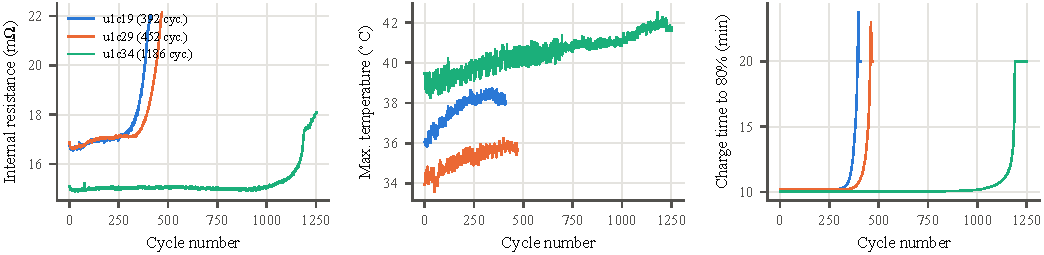
\includegraphics[width=\textwidth]{fig_summary_signals}
  \caption{Per-cycle summary signals for three cells: internal resistance
  (left), maximum cell temperature (middle) and charge time to 80\% SOC
  (right). Charge time saturates at 20\,min near EOL.}
  \label{fig:summary}
\end{figure*}

\subsection{Discharge curve and differential capacity}
Fig.~\ref{fig:qv}(a) shows how the discharge curve $Q(V)$ of \texttt{u1c0}
changes with ageing. The curve shrinks towards lower capacity and its
plateau sags to lower voltage, which reflects lost capacity and higher
resistance. Fig.~\ref{fig:qv}(b) shows the differential capacity
$\mathrm{d}Q/\mathrm{d}V$, whose main peak lies near 3.15\,V at the
\Crate{4} discharge rate. Ageing makes this peak smaller and shifts it to
lower voltage. Such changes are commonly used to identify the degradation
mode (LLI vs.\ LAM)~\cite{birkl2017}.

\begin{figure*}[t]
  \centering
  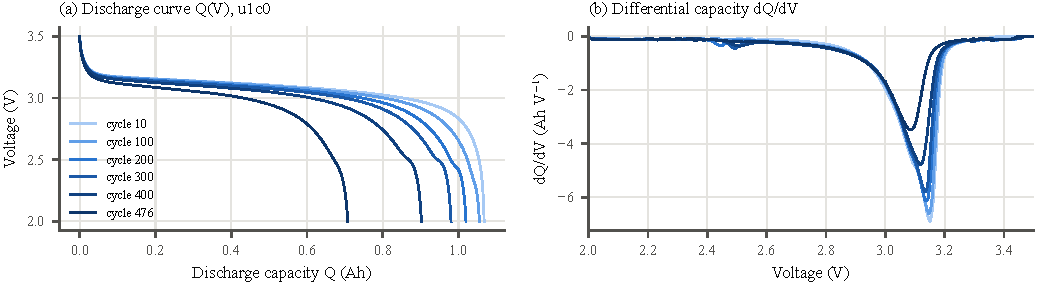
\includegraphics[width=\textwidth]{fig_qv_dqdv}
  \caption{(a) Discharge curve $Q(V)$ and (b) differential capacity
  $\mathrm{d}Q/\mathrm{d}V$ of \texttt{u1c0} at selected cycles. Darker
  lines are later cycles.}
  \label{fig:qv}
\end{figure*}

\subsection{The $\dq$ feature}
Following~\cite{severson2019}, we define
\begin{equation}
  \dq = Q_{100}(V) - Q_{10}(V),
\end{equation}
the difference between the discharge curves of cycles 100 and 10 on the
common \texttt{Vdlin} grid. This captures how the shape of the curve
changes early in life, even while total capacity has barely changed.
Fig.~\ref{fig:dq} plots it for all 39 cells.
\begin{itemize}
  \item Short-lived cells have large negative $\Delta Q$ (down to
  $-0.085$\,Ah) over the 2.8--3.1\,V range.
  \item Long-lived \texttt{-newstructure} cells have small $\Delta Q$,
  which is even slightly positive near 3.15\,V.
\end{itemize}

\begin{figure}[t]
  \centering
  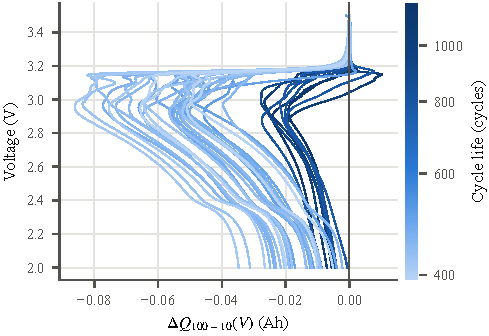
\includegraphics[width=\columnwidth]{fig_delta_q}
  \caption{$\dq$ for the 39 cells, coloured by cycle life. Cells that
  degrade faster show a larger negative shift.}
  \label{fig:dq}
\end{figure}

The summary statistic used in~\cite{severson2019} is
$\log_{10}\mathrm{Var}(\dq)$, the logarithm of the variance of $\dq$
across the 1000 voltage points. Fig.~\ref{fig:var} plots it against cycle
life. Table~\ref{tab:corr} gives the Pearson correlation with
$\log_{10}$(cycle life).

\begin{figure}[t]
  \centering
  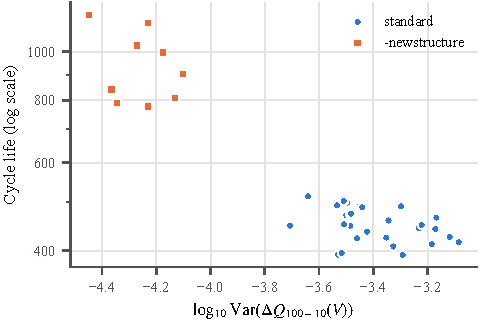
\includegraphics[width=\columnwidth]{fig_var_vs_life}
  \caption{$\log_{10}\mathrm{Var}(\dq)$ against cycle life (log scale). The
  overall trend is mostly explained by the separation between the two
  groups.}
  \label{fig:var}
\end{figure}

\begin{table}[t]
\centering
\caption{Pearson correlation between $\log_{10}\mathrm{Var}(\dq)$ and
$\log_{10}$(cycle life).}
\label{tab:corr}
\begin{tabular}{@{}lcc@{}}
\toprule
Subset & $n$ & $r$ \\
\midrule
All cells               & 39 & $-0.92$ \\
Standard only           & 30 & $-0.38$ \\
\texttt{-newstructure} only & 9 & $-0.27$ \\
\bottomrule
\end{tabular}
\end{table}

The strong overall correlation ($r=-0.92$) mainly reflects the difference
\emph{between} the two groups. \emph{Within} each group the relation is
weak. Part of the reason is that the cycle-life range inside each group is
narrow (392--514 for standard cells), so there is little variation for the
feature to explain. By contrast, the original study's data spans 150--2300
cycles~\cite{severson2019}. This is an important caveat for modelling, and
Section~\ref{sec:discussion} discusses it further.
